
\section{Définition et analyse de la chaine d'asservissement du robot esclave}
\begin{obj}
Définir le régulateur de la chaine d'asservissement du robot esclave, analyser ses performances vis-à-vis des perturbations en se limitant à celles dues aux couples de frottement sec et compléter la chaine d'asservissement par la compensation de ces efforts.
\end{obj}
\ifprof
\else
Un robot étant un système multivariable comportant en particulier des couplages entre les dynamiques des différents axes, la mise en place d'une loi de commande prenant en compte tous les axes peut se révéler complexe. Dans le cadre de ce sujet, on suppose

\begin{itemize}
  \item que des boucles internes locales à chaque axe motorisé ont été mises en place pour asservir le couple de chaque articulation à un couple de référence. Ceci permet de considérer le robot comme un système dont les entrées sont les couples moteurs intervenant dans les différentes articulations ;
  \item que des termes de compensation active des couples dus à la pesanteur ont été mis en place sur chaque articulation ;
  \item que les couplages entre les axes sont modélisés comme des entrées de perturbation dans les chaines d'asservissement.\\
L'objectif de cette partie est de déterminer la loi de commande permettant d'assurer l'asservissement de position des articulations $\theta_{32}$ et $\theta_{21}$ à des angles de référence issus du modèle cinématique inverse (figure \ref{fig_02}). Pour la suite de l'étude, on note les positions articulaires $q_{j}=\theta_{j}[j=32,21]$ et les consignes pour les chaines d'asservissement associées $q_{j}^{*}=\theta_{j}^{*}[j=32,21]$.
\end{itemize}
\fi

\subsection{Calcul d'un correcteur et analyse partielle des performances de la chaine d'asservissement}
\begin{obj}
Déterminer un correcteur pour la chaine d'asservissement de la position angulaire des articulations. Afin d'aboutir à une démarche générale (indépendante d'une articulation particulière), la loi de commande sera paramétrée par le moment d'inertie équivalent de l'articulation considérée.
\end{obj}

\ifprof
\else
Au regard des hypothèses précédentes, la synthèse du correcteur associé à une articulation $j$ peut être effectuée en utilisant le modèle suivant

$$
\indice{J}{eq} \ddot{q}_{j}(t)=c_{j}(t)+c_{\mathrm{ext}}(t)
$$

où $q_{j}$ est l'angle de rotation de l'articulation considérée, $\indice{J}{eq}$ est le moment d'inertie équivalent ramené sur l'axe de l'articulation $j, c_{j}$ est le couple moteur pour l'articulation considérée et $c_{\text {ext }}$ modélise un couple perturbateur représentant: les efforts de frottement sec, le couple dû à l'influence des autres axes et d'éventuels couples résiduels modélisant les incertitudes de compensation des effets de la gravité.

En supposant que les hypothèses précédentes sont validées, la chaine d'asservissement de l'articulation considérée est représentée par le schéma bloc de la figure \ref{fig_11} où $T(p)=Q_{j}(p) / C_{j}(p)$ est la fonction de transfert du couple de commande $c_{j}$ de l'articulation $j$ vers la position $q_{j}$ et où $K_{1}$ et $K_{2}$ sont les gains de la loi de commande choisie.

\begin{figure}[!h]
\centering
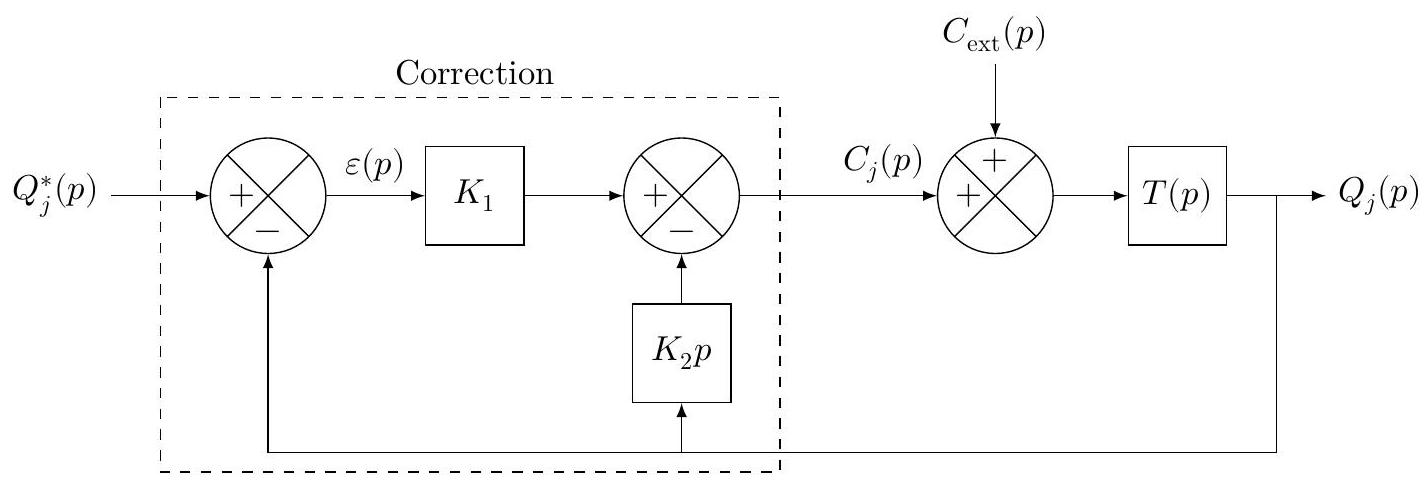
\includegraphics[width=.7\textwidth]{2024_08_29_b4f920ed3822451bf72bg-10}
\caption{\label{fig_11}Modèle de synthèse de la chaine d'asservissement d'une articulation}
\end{figure}

Les mesures disponibles étant réalisées au moyen de capteurs placés directement sur les motoréducteurs pour des questions de facilité de réalisation, on suppose que les grandeurs disponibles sont les positions angulaires des articulations. Pour cette raison, l'asservissement des axes est réalisé sur les mesures des positions angulaires des articulations et non directement sur les positions cartésiennes. Le cahier des charges partiel de cet asservissement est donné par le diagramme des exigences de la figure \ref{fig_12} déduit des exigences exprimées dans le repère cartésien du cahier des charges figure \ref{fig_03}.

\begin{figure}[!h]
\centering
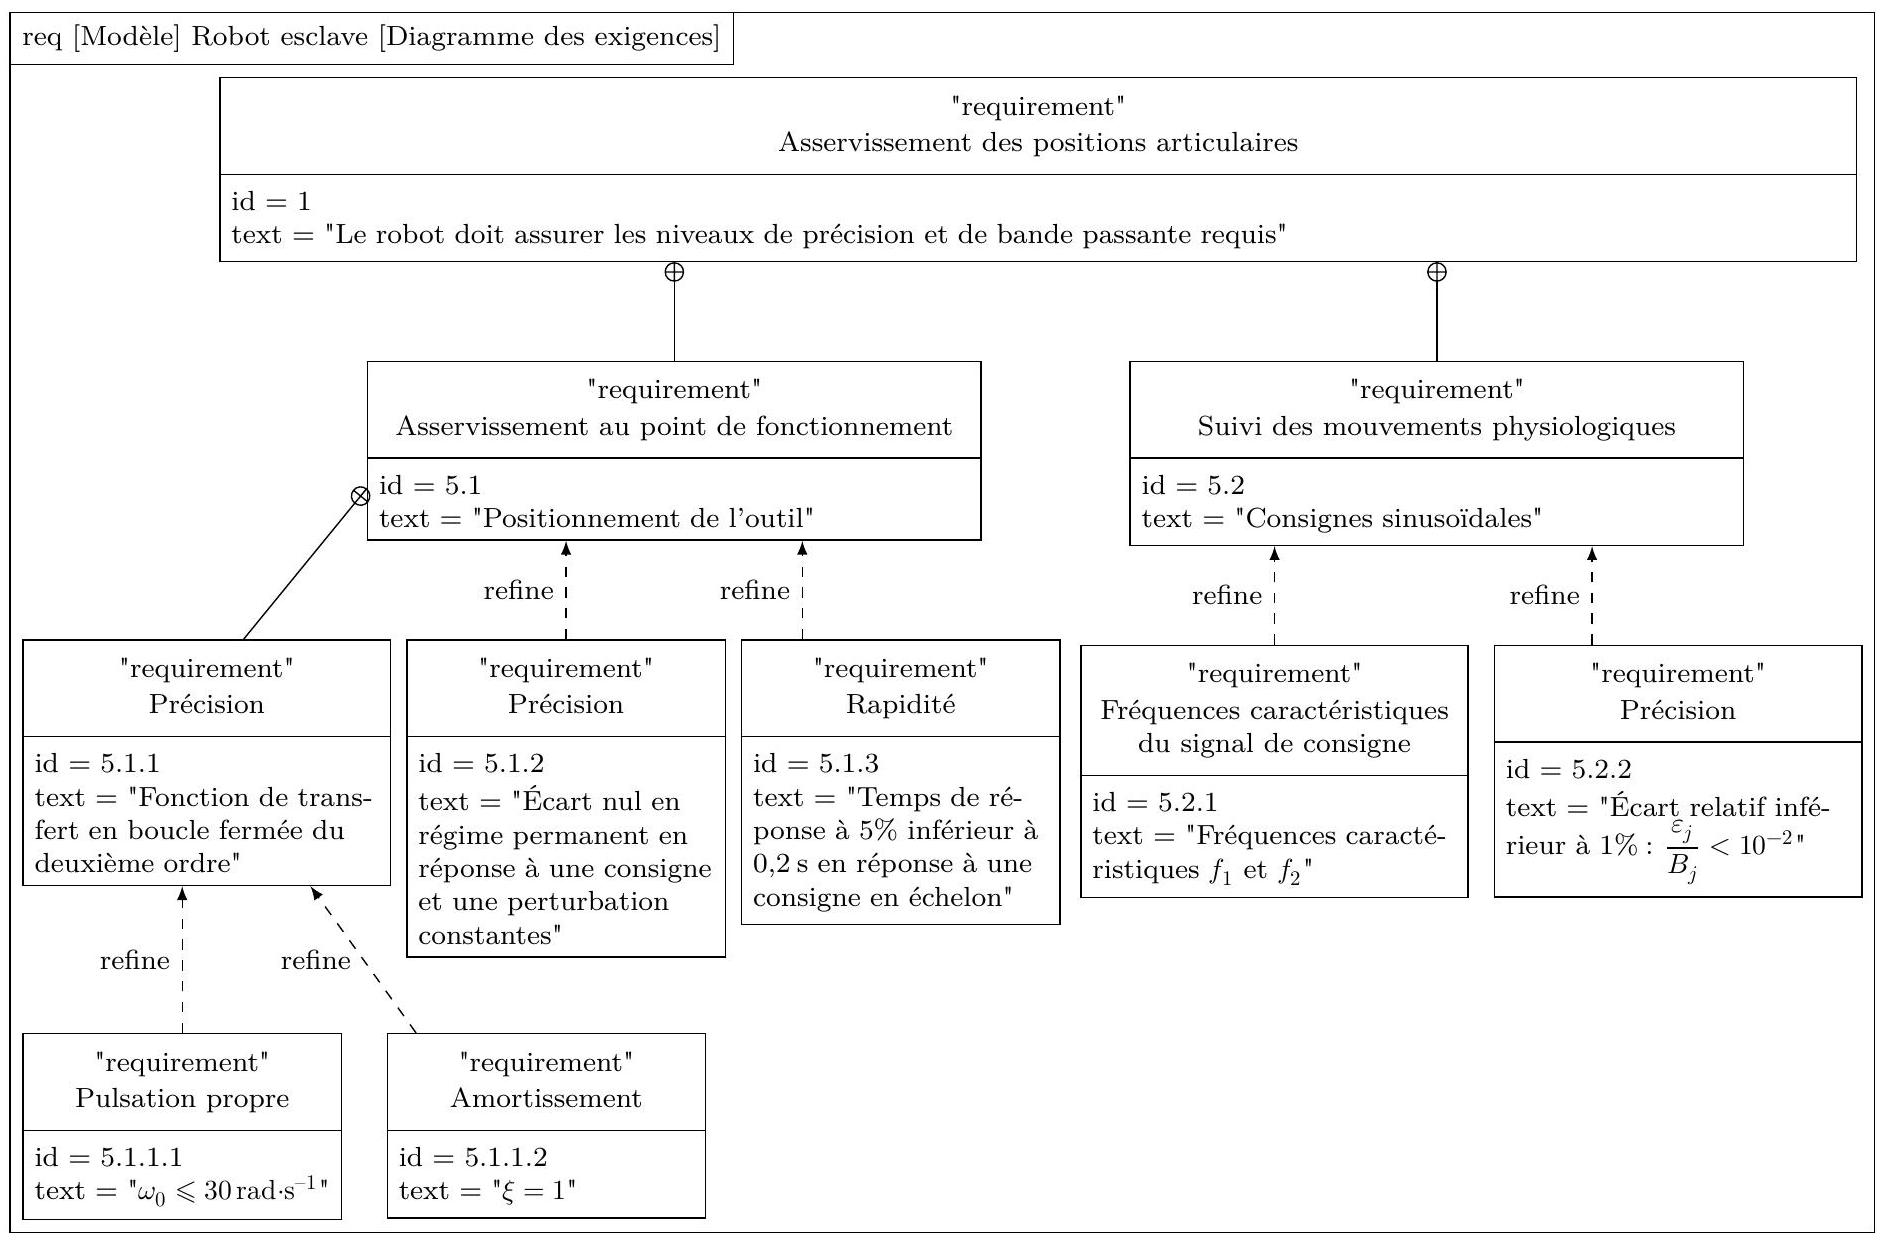
\includegraphics[max width=\textwidth]{2024_08_29_b4f920ed3822451bf72bg-11}
\caption{\label{fig_12}Diagramme des exigences de la chaine d'asservissement}
\end{figure}
\fi

%Q 24. 
\question{Déterminer l'expression de $T(p)$. Exprimer, sous forme canonique, la fonction de transfert en boucle fermée $F_{j}(p)=\frac{Q_{j}(p)}{Q_{j}^{*}(p)}$ en fonction de $\indice{J}{eq}, K_{1}$ et $K_{2}$. Déterminer alors les expressions littérales de $K_{1}$ et $K_{2}$ en fonction de $\indice{J}{eq}$, de la pulsation propre $\omega_{0}$ et de l'amortissement $\xi$ (exigence 5.1.1 du cahier des charges figure \ref{fig_12}).}
\ifprof
\begin{corrige}
En exprimant l'équation différentielle proposée dans le domaine de Laplace, on a 
$J_{\text{eq}} p^2{Q}_j(p)=C_j(p)+C_{\text{ext}}(p)$.
En utilisant le schéma-blocs, on a $Q_j(p)=\left(C_{\text{ext}}(p)+C_{\text{j}}(p)\right)T(p)$. 
Par analogie, on a donc $T(p)=\dfrac{1}{J_{\text{eq}}p^2}$.

On considère que $C_{\text{ext}}(p)=0$.  

On peut alors exprimer 
$F_j(p)= \dfrac{\dfrac{K_1T(p)}{1+T(p)K_2 p} }{1+\dfrac{K_1T(p)}{1+T(p)K_2 p}}$
$= \dfrac{\dfrac{K_1T(p)}{1+T(p)K_2 p} }{1+\dfrac{K_1T(p)}{1+T(p)K_2 p}}$
$= \dfrac{K_1T(p) }{1+T(p)K_2 p+K_1T(p)}$

$= \dfrac{K_1\dfrac{1}{J_{\text{eq}}p^2}}{1+\dfrac{1}{J_{\text{eq}}p^2}K_2 p+K_1\dfrac{1}{J_{\text{eq}}p^2}}$

$= \dfrac{K_1}{J_{\text{eq}}p^2+K_2 p+K_1}$

$= \dfrac{1}{\dfrac{J_{\text{eq}}}{K_1}p^2+\dfrac{K_2}{K_1}p+1}$.

On a donc $\dfrac{1}{\omega_0^2}=\dfrac{J_{\text{eq}}}{K_1}$ et $\dfrac{2\xi}{\omega_0}=\dfrac{K_2}{K_1}$. On a donc $K_1=J_{\text{eq}}\omega_0^2$ et $K_2=\dfrac{2\xi K_1}{\omega_0}=2\xi J_{\text{eq}}\omega_0$.
\end{corrige}
\else
\fi

\ifprof
\else
Un des problèmes majeurs de ce type de robot, surtout aux faibles vitesses de déplacement, est la présence d'efforts de frottement sec de valeur importante qui peuvent se traduire par des oscillations aux faibles vitesses ou encore par des erreurs en régime permanent. Pour l'analyse en régime permanent, une solution est de modéliser ce type d'effort comme un signal perturbateur externe constant.\\
\fi

%Q 25. 
\question{En conservant les gains $K_{1}$ et $K_{2}$ déterminés précédemment, préciser la fonction de transfert en boucle fermée $D(p)=\frac{Q_{j}(p)}{C_{\text {ext }}(p)}$ en fonction de $\indice{J}{eq}, \omega_{0}$ et $\xi$. Déterminer alors littéralement l'écart en régime permanent, $\lim\limits_{t \rightarrow+\infty} \varepsilon(t)$, pour une variation en échelon de l'effort perturbateur $c_{\text {ext }}(t)=C_{\text {ext } 0} \Upsilon(t)$ d'amplitude $C_{\text {ext } 0}$ où $\Upsilon(t)$ représente l'échelon d'Heaviside. Conclure sur la performance associée.}
\ifprof
\begin{corrige}
On imagine ici qu'il faut considérer que $Q*_j(p)=0$.

On a $C_j(p)=-\left(K_1+K_2 p\right) Q_j(p)$ et $Q_j(p)=\left(C_j(p)+C_{\text{ext}}(p)\right)T(p)$.  On a donc  

%$Q_j(p)=\left(-\left(K_1+K_2 p\right) Q_j(p)+C_{\text{ext}}(p)\right)T(p)$
%$\Leftrightarrow \left(1-\left(K_1+K_2 p\right)T(p) \right)Q_j(p)=C_{\text{ext}}(p)$
%$\Leftrightarrow \dfrac{Q_j(p)}{C_{\text{ext}}(p)}=\dfrac{1}{1-\left(K_1+K_2 p\right)T(p) }$.


$Q_j(p)=\left(-\left(K_1+K_2 p\right) Q_j(p)+C_{\text{ext}}(p)\right)T(p)$
$\Leftrightarrow \left(1+\left(K_1+K_2 p\right)T(p) \right)Q_j(p)=C_{\text{ext}}(p)\cdot T(p)$

$\Leftrightarrow \dfrac{Q_j(p)}{C_{\text{ext}}(p)}=\dfrac{T(p)}{1+\left(K_1+K_2 p\right)T(p) }$.

En utilisant les valeurs déterminées précédemment, on a donc $D(p)=\dfrac{\dfrac{1}{\indice{J}{eq}p^2}}{1+\left(J_{\text{eq}}\omega_0^2+2\xi J_{\text{eq}}\omega_0 p\right)\dfrac{1}{J_{\text{eq}}p^2} }$

$=\dfrac{1}{\indice{J}{eq}p^2+2\xi J_{\text{eq}}\omega_0 p+\indice{J}{eq}\omega_0^2}=\dfrac{\dfrac{1}{\indice{J}{eq}\omega_0^2}}{\dfrac{p^2}{\omega_0^2}+\dfrac{2\xi}{\omega_0}p+1}$.

On a $C_{\text{ext}}(p)=\dfrac{C_{\text{ext} 0}}{p}$. En conséquence, 
$\lim\limits_{t\to +\infty} \varepsilon(t) = \lim\limits_{p\to 0} p\varepsilon(p)$.
Par ailleurs,  $\varepsilon(p)=-Q_j(p)=-D(p)C_{\text{ext}}(p)$.

On a alors $\lim\limits_{t\to +\infty} \varepsilon(t) = \lim\limits_{p\to 0} -pD(p)C_{\text{ext}}(p)= \lim\limits_{p\to 0} -p\dfrac{\dfrac{1}{\indice{J}{eq}\omega_0^2}}{\dfrac{p^2}{\omega_0^2}+\dfrac{2\xi}{\omega_0}p+1}\cdot \dfrac{C_{\text{ext0}}}{p}$
$=  -\dfrac{C_{\text{ext} 0}}{\indice{J}{eq}\omega_0^2}$.

\textbf{Conclusion :} l'erreur ici n'est pas nulle et elle dépend de l'inertie, de la pulsation propre $\omega_0$ et de l'amplitude de la perturbation. 
\end{corrige}
\else
\fi


%III.B - 
\subsection{Amélioration des performances par compensation du couple de perturbation}
%Objectif\\
\begin{obj}
Améliorer les performances de la loi de commande vis-à-vis des couples perturbateurs extérieurs.
\end{obj}

\ifprof
\else

Une solution pour améliorer la performance en précision serait de compléter le correcteur en introduisant un terme intégral. Cependant, l'introduction de ce terme diminuera les marges de stabilité et son calcul peut s'avérer difficile au regard de la fonction de transfert en boucle ouverte s'il est nécessaire d'assurer un certain niveau de performance dynamique.

Une solution alternative est de compenser le terme perturbateur en introduisant une loi de commande $c_{j}(t)=$ $\tilde{c}_{j}(t)-c_{\text {ext }}(t)$ (soit après compensation, un modèle du procédé à considérer $\indice{J}{eq} \ddot{q}_{j}(t)=\tilde{c}_{j}(t)$ ne faisant pas apparaître de terme perturbateur). Cependant, cette solution nécessite de disposer de la mesure du signal perturbateur, irréalisable en pratique. Afin de répondre à ce problème, une solution est de mettre en place un observateur permettant d'obtenir une estimée $\hat{c}_{\text {ext }}(t)$ du couple extérieur. Cet observateur est mis en place en utilisant les relations suivantes

$$
\left\{\begin{array}{l}
\hat{Q}_{j}(p)=T(p)\left(C_{j}(p)+\hat{C}_{\mathrm{ext}}(p)\right) \\
\hat{C}_{\mathrm{ext}}(p)=K(p)\left(Q_{j}(p)-\hat{Q}_{j}(p)\right)
\end{array}\right.
$$

où $K(p)$ est un correcteur à déterminer et $\hat{Q}_{j}(p)$ une estimation de $Q_{j}(p)$.\\
\fi

%Q 26. 
\question{En utilisant ces équations, compléter le schéma bloc modélisant cet observateur (figure \ref{fig_B} du document réponse).}
\ifprof
\begin{corrige}
\begin{rem}
Il semblerait qu'il manque une information concernant le schéma bloc. Il faudrait sans doute ajouter $\hat{Q}_j(p)$. Cela donnerait la figure suivante.
\end{rem}

\begin{center}
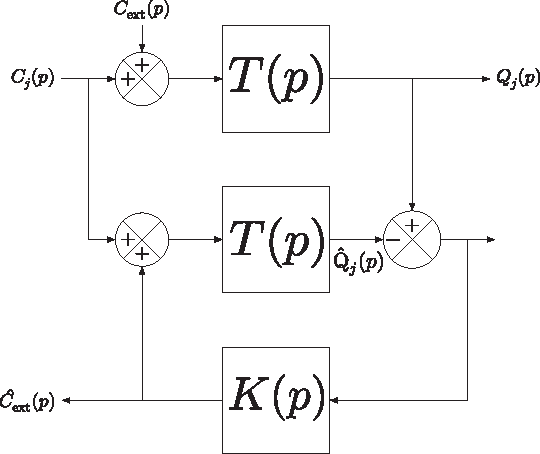
\includegraphics[width=0.4\textwidth]{DR_B_corrige.pdf}
\end{center}
\end{corrige}
\else
\fi

%Q27
\question{Au moyen d'une approche à choisir, montrer que le schéma bloc de la figure \ref{fig_B} , représentatif de l'observateur, peut être réduit au schéma bloc équivalent de la figure \ref{fig_13}.}
\ifprof
\begin{corrige}
En manipulant le schéma bloc on peut obtenir : 

\begin{center}
\begin{tabular}{cc}
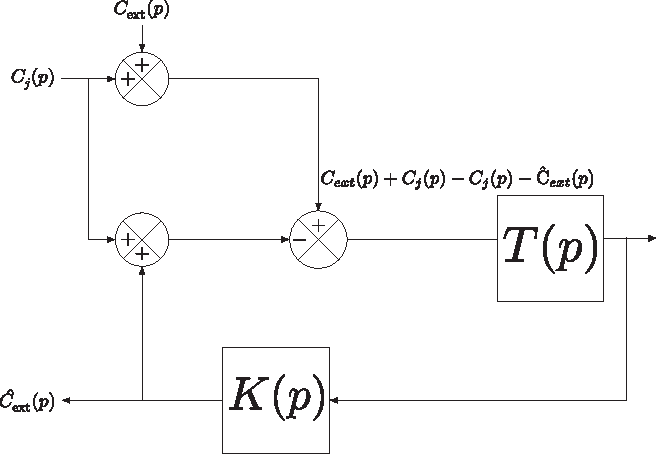
\includegraphics[width=0.5\textwidth]{DR_B_corrige2.pdf}
&
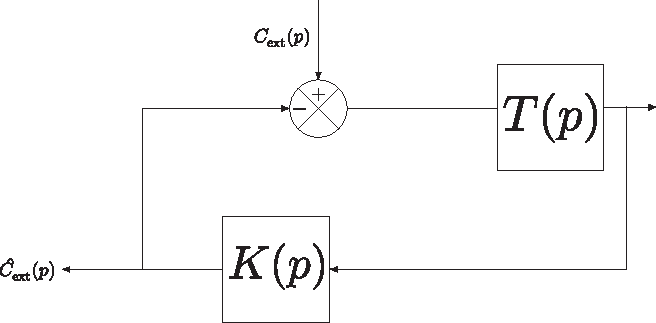
\includegraphics[width=0.5\textwidth]{DR_B_corrige3.pdf}
\end{tabular}
\end{center}

En permutant les blocs $T(p)$ et $K(p)$ qui sont en série on obtient la forme souhaitée.

\end{corrige}
\else
\fi


\begin{figure}[!h]
\centering
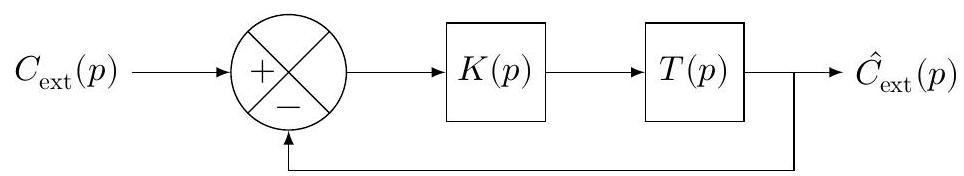
\includegraphics[width=.6\textwidth]{2024_08_29_b4f920ed3822451bf72bg-12}
\caption{\label{fig_13} Modèle équivalent de l'estimateur du couple perturbateur}
\end{figure}


Le calcul du correcteur $K(p)$ peut être alors effectué en utilisant le schéma bloc de la figure \ref{fig_13} où $C_{\text {ext }}(p)$ peut être interprété comme une consigne fictive.

%Q 28. 
\question{En adoptant une démarche comparable à celle utilisée dans la sous-partie III.A, proposer la fonction de transfert d'un correcteur $K(p)$ à deux paramètres, notés $K_{1}^{\prime}$ et $K_{2}^{\prime}$, de façon à ce que la fonction de transfert en boucle fermée ait un polynôme caractéristique du second ordre $\left(p+\omega_{0}^{\prime}\right)^{2}$, d'amortissement $\xi=1$ et de pulsation propre $\omega_{0}^{\prime}=5 \omega_{0}$. Exprimer littéralement ces deux paramètres en fonction de $\indice{J}{eq}, \omega_{0}$ et $\xi$. On s'attachera à justifier brièvement que l'erreur en régime permanent est nulle vis-à-vis d'un couple $c_{\text {ext }}$ constant, c'est à dire que $\lim\limits_{t \rightarrow \infty}\left(c_{\text {ext }}(t)-\hat{c}_{\text {ext }}(t)\right)=0$ en réponse à une variation en échelon du couple perturbateur $c_{\text {ext }}(t)=C_{\text {ext } 0} \Upsilon(t)$.}
\ifprof
\begin{corrige}

\textbf{Remarque : } on peut hésiter entre prendre la structure de la partie III.A (Méthode A) ou donner un $K(p)$ équivalent sous la forme d'un correcteur P.D. (Méthode B).

%\begin{minipage}[t]{0.4\textwidth}
\begin{multicols}{2}
\textbf{Méthode A :}
Ainsi en manipulant le schéma bloc on obtient : 

\begin{center}
%\begin{large}
\begin{tikzpicture}
\sbEntree{E0}
\sbComp[4]{c2}{E0}
\sbRelier[$C_{\text{ext}}(p)$]{E0}{c2}
\sbBloc[1]{b2}{$K'_1$}{c2}
\sbRelier{c2}{b2}
\sbBloc[3]{b4}{$T(p)$}{b2}
\sbRelier[]{b2}{b4}
\sbSortie[4]{S}{b4}
\sbRelier[\^{C}$_{\text{ext}}(p)$]{b4}{S}
\sbDecaleNoeudy[4]{S}{v}
\sbBlocr[4]{b10}{$1+\frac{K'_2\cdot p}{K'_1}$}{v}
%\sbBlocr[4]{b10}{$1+\frac{K_'2\cdot p}{K'_1}$}{v}
\sbRelieryx{b4-S}{b10}
\sbRelierxy[]{b10}{c2}
\end{tikzpicture}
%\end{large}
\end{center}

La fonction de transfert en boucle fermée est donnée par : 

$
H_{BF}(p)=\dfrac{\dfrac{K'_1}{\indice{J}{eq}p^2}}{1+\dfrac{K'_1}{\indice{J}{eq}p^2}\left(1+\dfrac{K'_2}{K'_1}p\right)}$

$=
\dfrac{K'_1}{\indice{J}{eq}\cdot p^2+K'_2\cdot p+K'_1}$

$=\dfrac{1}{1+\dfrac{K'_2}{K'_1}p+\dfrac{\indice{J}{eq}}{K'_1}p^2}
$



\textbf{Méthode B :}

Ainsi en manipulant le schéma bloc on obtient : 

\begin{center}
%\begin{large}
\begin{tikzpicture}
\sbEntree{E0}
\sbComp[4]{c2}{E0}
\sbRelier[$C_{\text{ext}}(p)$]{E0}{c2}
\sbBloc[1]{b2}{$K'_1+K'_2\cdot p$}{c2}
\sbRelier{c2}{b2}
\sbBloc[3]{b4}{$T(p)$}{b2}
\sbRelier[]{b2}{b4}
\sbSortie[4]{S}{b4}
\sbRelier[\^{C}$_{\text{ext}}(p)$]{b4}{S}
\sbDecaleNoeudy[4]{S}{v}
\sbBlocr[4]{b10}{$1$}{v}
%\sbBlocr[4]{b10}{$1+\frac{K_'2\cdot p}{K'_1}$}{v}
\sbRelieryx{b4-S}{b10}
\sbRelierxy[]{b10}{c2}
\end{tikzpicture}
%\end{large}
\end{center}

La fonction de transfert en boucle fermée est donnée par : 

$
H_{BF}(p)=\dfrac{\dfrac{K'_1+K'_2\cdot p}{\indice{J}{eq}p^2}}{1+\dfrac{K'_1+K'_2\cdot p}{\indice{J}{eq}p^2}}$
$ =\dfrac{K'_1+K'_2\cdot p}{\indice{J}{eq}\cdot p^2+K'_2\cdot p+K'_1}$
$=\dfrac{1+\dfrac{K'_2}{K'_1}p}{1+\dfrac{K'_2}{K'_1}p+\dfrac{\indice{J}{eq}}{K'_1}p^2}$.

%\end{minipage}
\end{multicols}
Par identification, pour les deux méthodes et avec ce qu'impose la cahier des charges.

$
\left\{
\begin{array}{c}
\omega'_0=\sqrt{\dfrac{K'_1}{\indice{J}{eq}}}=5\omega_0\\
\\
\xi=\dfrac{\omega'_0}{2}\dfrac{K'_2}{K'_1}=\dfrac{1}{2}\sqrt{\dfrac{K'_1}{\indice{J}{eq}}}\dfrac{K'_2}{K'_1}=1
\end{array}
\right.
$. 
On obtient alors,
$
\left\{
\begin{array}{c}
K'_1=25\cdot \indice{J}{eq}\cdot \omega_0^2\\
\\
K'_2=2\sqrt{K'_1\cdot \indice{J}{eq}}=10\cdot \indice{J}{eq}\cdot \omega_0
\end{array}
\right.
$.

\textbf{La fonction de transfert en boucle ouverte est de classe 2 ainsi l'erreur statique est nulle. }
\end{corrige}
\else
\fi

\ifprof
\else

Cette première structure de commande correspondant à la relation

$$
C_{j}(p)=\tilde{C}_{j}(p)-\hat{C}_{\text {ext }}(p)=\left(K_{1}\left(Q_{j}^{*}(p)-Q_{j}(p)\right)-K_{2} p Q_{j}(p)\right)-\hat{C}_{\text {ext }}(p)
$$

peut être représentée par le schéma bloc de la figure \ref{fig_14}. Elle sera conservée et complétée dans la suite de l'étude.


\begin{figure}[!h]
\centering
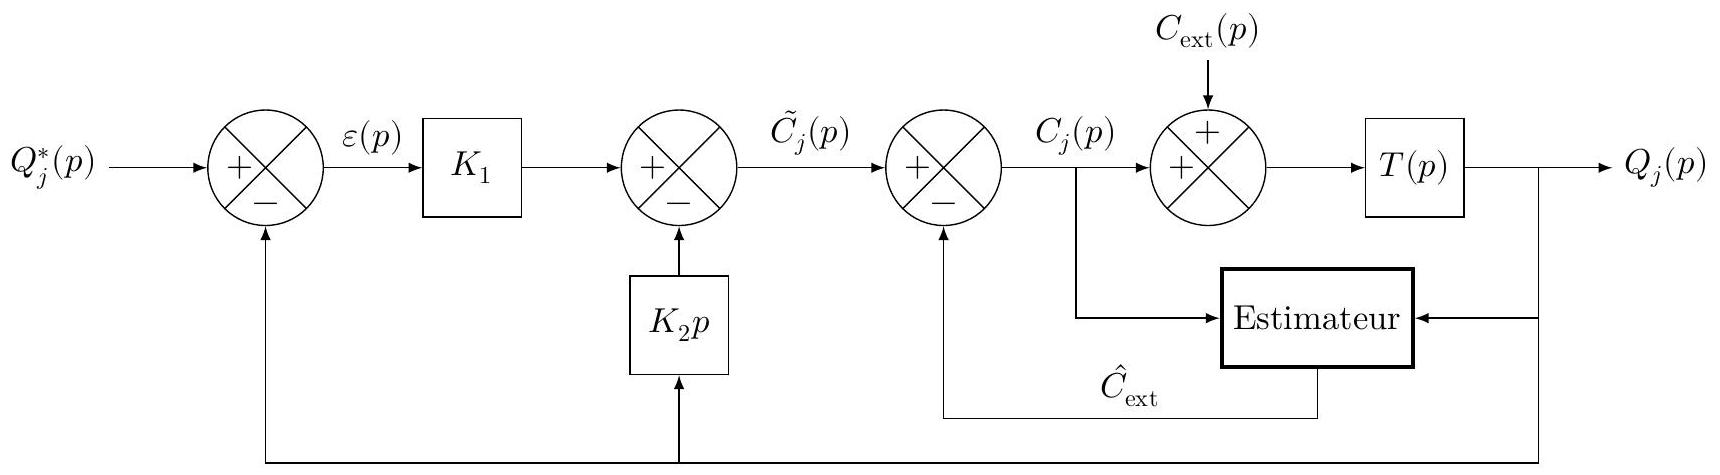
\includegraphics[width=.9\textwidth]{2024_08_29_b4f920ed3822451bf72bg-12(1)}
\caption{\label{fig_14} Schéma bloc de la commande avec estimation et compensation de couple perturbateur}
\end{figure}


L'introduction de la compensation $C_{j}(p)=\left(K_{1}\left(Q_{j}^{*}(p)-Q_{j}(p)\right)-K_{2} p Q_{j}(p)\right)-\hat{C}_{\text {ext }}(p)$ de la perturbation modifie la structure de la boucle et la stabilité en boucle fermée n'est plus garantie à priori.
\fi

%Q 29. 
\question{En utilisant cette compensation, déterminer la fonction de transfert $\frac{Q_{j}(p)}{C_{\text {ext }}}$ et l'exprimer en fonction de $T(p), K_{1}, K_{2}$ et $K(p)$ (on supposera que la consigne est nulle $Q_{j}^{*}=0$ et que le système est bouclé par le correcteur déterminé à la sous-partie III.A). En déduire le polynôme caractéristique puis, en justifiant la réponse, conclure sur la stabilité du système bouclé et sur l'écart en régime permanent lorsque le couple perturbateur $c_{\text {ext }}$ est constant.}
\ifprof
\begin{corrige}

Notons $H_{28}(p)$ la fonction de transfert déterminée à la question 28 :  $
H_{28}(p)=\dfrac{\text{\^{C}}_{\text{ext}}(p)}{C_{\text{ext}}(p)}=\dfrac{K(p)\cdot T(p)}{1+K(p)\cdot T(p)}$.

Avec $Q^*_j(p)=0$, $
C_j(p)=\text{\~{C}}_j(p)-\text{\^{C}}_{ext}(p)=-\left(K_1+K_2\cdot p\right)Q_j(p)-H_{28}(p)C_{\text{ext}}(p)\\
$.

D'après la lecture du schéma bloc : 

$Q_j(p)=T(p)\left(C_j(p)+C_{\text{ext}}(p)\right)=T(p)\left(-\left(K_1+K_2\cdot p\right)Q_j(p)+\left(1-H_{28}(p)\right)C_{\text{ext}}(p)\right) $
$ \Leftrightarrow 
Q_j(p)\left(1+T(p)\left(K_1+K_2\cdot p\right)\right)=C_{\text{ext}}(p)T(p)\left(1-H_{28}(p)\right)$.

On trouve donc : $
\dfrac{Q_j(p)}{C_{\text{ext}}(p)}=\dfrac{T(p)}{\left(1+K(p)\cdot T(p)\right)\left(1+T(p)\left(K_1+K_2\cdot p\right)\right)}
$.

Avec $K(p)=K'_1+K'_2\cdot p$ et $T(p)=\dfrac{1}{\indice{J}{eq}p^2}$,
$
\dfrac{Q_j(p)}{C_{\text{ext}}(p)}=\dfrac{\indice{J}{eq}p^2}{\left(\indice{J}{eq}p^2+K'_1+K'_2\cdot p\right)\left(\indice{J}{eq}p^2+K_1+K_2\cdot p\right)}
$.

D'après les questions 24 et 27,
$
\dfrac{Q_j(p)}{C_{\text{ext}}(p)}=\dfrac{\dfrac{p^2}{\indice{J}{eq}}}{\left(p+\omega'_0\right)^2\left(p+\omega_0\right)^2}
$.



\begin{itemize}
\item \textbf{Stabilité : } on remarque que les pôles de la FTBF sont à partie réelles strictement négatives ($-\omega_0$ et $-\omega'_0$) ce qui \textbf{est une condition nécessaire et suffisante de stabilité.}
\item \textbf{Précision : } soit $\varepsilon(p)$ $=-Q_j(p)$ $=-\dfrac{\dfrac{p^2}{\indice{J}{eq}}}{\left(p+\omega'_0\right)^2\left(p+\omega_0\right)^2}C_{\text{ext}}(p)$. En considérant $C_{\text{ext}}$ comme une constante, $C_{\text{ext}}(p)=\dfrac{C_0}{p}$. 
L'erreur statique vis-à-vis d'une perturbation constante est donnée par :
$\varepsilon_s= \lim\limits_{p\rightarrow0} p\varepsilon(p)$ $= \lim\limits_{p\rightarrow0}\left[-\dfrac{\dfrac{C_0\cdot p^2}{\indice{J}{eq}}}{\left(p+\omega'_0\right)^2\left(p+\omega_0\right)^2}\right]=0
$.

\textbf{L'erreur statique vis-à-vis d'une perturbation constante est bien nulle.}
\end{itemize}

\end{corrige}
\else
\fi
